% Generated by benchmarks/src/utils/make_table4_speedup_figures.py -- do not hand-edit.
\definecolor{sp0}{HTML}{2A78D6}
\definecolor{sp1}{HTML}{EB6834}
\definecolor{sp2}{HTML}{1BAF7A}
\pgfdeclareplotmark{heptagon*}{\pgfpathmoveto{\pgfqpointpolar{90.00}{\pgfplotmarksize}}\pgfpathlineto{\pgfqpointpolar{141.43}{\pgfplotmarksize}}\pgfpathlineto{\pgfqpointpolar{192.86}{\pgfplotmarksize}}\pgfpathlineto{\pgfqpointpolar{244.29}{\pgfplotmarksize}}\pgfpathlineto{\pgfqpointpolar{295.71}{\pgfplotmarksize}}\pgfpathlineto{\pgfqpointpolar{347.14}{\pgfplotmarksize}}\pgfpathlineto{\pgfqpointpolar{38.57}{\pgfplotmarksize}}\pgfpathclose\pgfusepathqfill}
\pgfdeclareplotmark{octagon*}{\pgfpathmoveto{\pgfqpointpolar{90.00}{\pgfplotmarksize}}\pgfpathlineto{\pgfqpointpolar{135.00}{\pgfplotmarksize}}\pgfpathlineto{\pgfqpointpolar{180.00}{\pgfplotmarksize}}\pgfpathlineto{\pgfqpointpolar{225.00}{\pgfplotmarksize}}\pgfpathlineto{\pgfqpointpolar{270.00}{\pgfplotmarksize}}\pgfpathlineto{\pgfqpointpolar{315.00}{\pgfplotmarksize}}\pgfpathlineto{\pgfqpointpolar{0.00}{\pgfplotmarksize}}\pgfpathlineto{\pgfqpointpolar{45.00}{\pgfplotmarksize}}\pgfpathclose\pgfusepathqfill}
\begin{figure*}[!t]
    \centering
    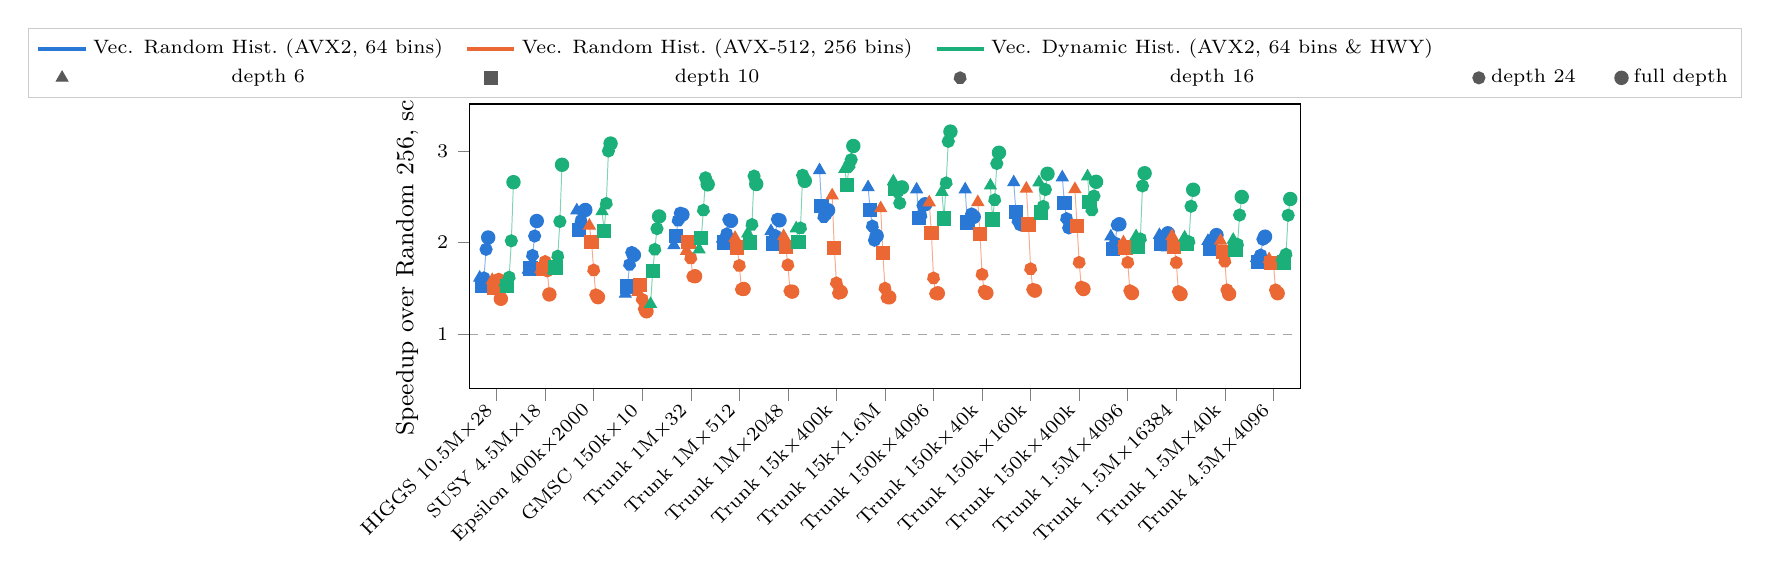
\begin{tikzpicture}
    \begin{axis}[
        width=\textwidth, height=5.2cm,
        xmin=0.45, xmax=17.55,
        ymin=0.41, ymax=3.51,
        xtick={1,2,3,4,5,6,7,8,9,10,11,12,13,14,15,16,17},
        xticklabels={HIGGS 10.5M$\times$28, SUSY 4.5M$\times$18, Epsilon 400k$\times$2000, GMSC 150k$\times$10, Trunk 1M$\times$32, Trunk 1M$\times$512, Trunk 1M$\times$2048, Trunk 15k$\times$400k, Trunk 15k$\times$1.6M, Trunk 150k$\times$4096, Trunk 150k$\times$40k, Trunk 150k$\times$160k, Trunk 150k$\times$400k, Trunk 1.5M$\times$4096, Trunk 1.5M$\times$16384, Trunk 1.5M$\times$40k, Trunk 4.5M$\times$4096},
        xticklabel style={rotate=45, anchor=east, font=\scriptsize},
        yticklabel style={font=\scriptsize},
        ylabel={Speedup over Random 256, scalar},
        ylabel style={font=\small},
        tick align=outside, tick pos=left,
        legend columns=5, legend style={font=\scriptsize, draw=gray!40,
            at={(0.5,1.02)}, anchor=south, /tikz/every even column/.append style={column sep=6pt}},
    ]
    \addplot[color=sp0, line width=0.35pt, opacity=0.55, mark=none, forget plot] coordinates {(0.652,1.6194) (0.696,1.5355) (0.740,1.6178) (0.784,1.9281) (0.828,2.0571)};
    \addplot[color=sp0, line width=0.35pt, opacity=0.55, mark=none, forget plot] coordinates {(1.652,1.7055) (1.696,1.7206) (1.740,1.8622) (1.784,2.0731) (1.828,2.2363)};
    \addplot[color=sp0, line width=0.35pt, opacity=0.55, mark=none, forget plot] coordinates {(2.652,2.3513) (2.696,2.1402) (2.740,2.2394) (2.784,2.3449) (2.828,2.3568)};
    \addplot[color=sp0, line width=0.35pt, opacity=0.55, mark=none, forget plot] coordinates {(3.652,1.4443) (3.696,1.5254) (3.740,1.7630) (3.784,1.8943) (3.828,1.8665)};
    \addplot[color=sp0, line width=0.35pt, opacity=0.55, mark=none, forget plot] coordinates {(4.652,1.9726) (4.696,2.0750) (4.740,2.2423) (4.784,2.3220) (4.828,2.3068)};
    \addplot[color=sp0, line width=0.35pt, opacity=0.55, mark=none, forget plot] coordinates {(5.652,2.0435) (5.696,2.0009) (5.740,2.0965) (5.784,2.2511) (5.828,2.2381)};
    \addplot[color=sp0, line width=0.35pt, opacity=0.55, mark=none, forget plot] coordinates {(6.652,2.1261) (6.696,1.9921) (6.740,2.0792) (6.784,2.2551) (6.828,2.2441)};
    \addplot[color=sp0, line width=0.35pt, opacity=0.55, mark=none, forget plot] coordinates {(7.652,2.7887) (7.696,2.3995) (7.740,2.2817) (7.784,2.3118) (7.828,2.3539)};
    \addplot[color=sp0, line width=0.35pt, opacity=0.55, mark=none, forget plot] coordinates {(8.652,2.6035) (8.696,2.3576) (8.740,2.1814) (8.784,2.0273) (8.828,2.0743)};
    \addplot[color=sp0, line width=0.35pt, opacity=0.55, mark=none, forget plot] coordinates {(9.652,2.5792) (9.696,2.2688) (9.740,2.2937) (9.784,2.4046) (9.828,2.4188)};
    \addplot[color=sp0, line width=0.35pt, opacity=0.55, mark=none, forget plot] coordinates {(10.652,2.5803) (10.696,2.2188) (10.740,2.2321) (10.784,2.3137) (10.828,2.2827)};
    \addplot[color=sp0, line width=0.35pt, opacity=0.55, mark=none, forget plot] coordinates {(11.652,2.6576) (11.696,2.3367) (11.740,2.2365) (11.784,2.1971) (11.828,2.1992)};
    \addplot[color=sp0, line width=0.35pt, opacity=0.55, mark=none, forget plot] coordinates {(12.652,2.7112) (12.696,2.4336) (12.740,2.2628) (12.784,2.1616) (12.828,2.1847)};
    \addplot[color=sp0, line width=0.35pt, opacity=0.55, mark=none, forget plot] coordinates {(13.652,2.0680) (13.696,1.9301) (13.740,1.9984) (13.784,2.1933) (13.828,2.2014)};
    \addplot[color=sp0, line width=0.35pt, opacity=0.55, mark=none, forget plot] coordinates {(14.652,2.0835) (14.696,1.9846) (14.740,1.9722) (14.784,2.0799) (14.828,2.1028)};
    \addplot[color=sp0, line width=0.35pt, opacity=0.55, mark=none, forget plot] coordinates {(15.652,2.0191) (15.696,1.9304) (15.740,1.9577) (15.784,2.0458) (15.828,2.0830)};
    \addplot[color=sp0, line width=0.35pt, opacity=0.55, mark=none, forget plot] coordinates {(16.652,1.8334) (16.696,1.7937) (16.740,1.8668) (16.784,2.0380) (16.828,2.0664)};
    \addplot[color=sp0, mark=triangle*, mark size=2.4pt, only marks, forget plot] coordinates {(0.652,1.6194) (1.652,1.7055) (2.652,2.3513) (3.652,1.4443) (4.652,1.9726) (5.652,2.0435) (6.652,2.1261) (7.652,2.7887) (8.652,2.6035) (9.652,2.5792) (10.652,2.5803) (11.652,2.6576) (12.652,2.7112) (13.652,2.0680) (14.652,2.0835) (15.652,2.0191) (16.652,1.8334)};
    \addplot[color=sp0, mark=square*, mark size=2.4pt, only marks, forget plot] coordinates {(0.696,1.5355) (1.696,1.7206) (2.696,2.1402) (3.696,1.5254) (4.696,2.0750) (5.696,2.0009) (6.696,1.9921) (7.696,2.3995) (8.696,2.3576) (9.696,2.2688) (10.696,2.2188) (11.696,2.3367) (12.696,2.4336) (13.696,1.9301) (14.696,1.9846) (15.696,1.9304) (16.696,1.7937)};
    \addplot[color=sp0, mark=heptagon*, mark size=2.4pt, only marks, forget plot] coordinates {(0.740,1.6178) (1.740,1.8622) (2.740,2.2394) (3.740,1.7630) (4.740,2.2423) (5.740,2.0965) (6.740,2.0792) (7.740,2.2817) (8.740,2.1814) (9.740,2.2937) (10.740,2.2321) (11.740,2.2365) (12.740,2.2628) (13.740,1.9984) (14.740,1.9722) (15.740,1.9577) (16.740,1.8668)};
    \addplot[color=sp0, mark=octagon*, mark size=2.4pt, only marks, forget plot] coordinates {(0.784,1.9281) (1.784,2.0731) (2.784,2.3449) (3.784,1.8943) (4.784,2.3220) (5.784,2.2511) (6.784,2.2551) (7.784,2.3118) (8.784,2.0273) (9.784,2.4046) (10.784,2.3137) (11.784,2.1971) (12.784,2.1616) (13.784,2.1933) (14.784,2.0799) (15.784,2.0458) (16.784,2.0380)};
    \addplot[color=sp0, mark=*, mark size=2.4pt, only marks, forget plot] coordinates {(0.828,2.0571) (1.828,2.2363) (2.828,2.3568) (3.828,1.8665) (4.828,2.3068) (5.828,2.2381) (6.828,2.2441) (7.828,2.3539) (8.828,2.0743) (9.828,2.4188) (10.828,2.2827) (11.828,2.1992) (12.828,2.1847) (13.828,2.2014) (14.828,2.1028) (15.828,2.0830) (16.828,2.0664)};
    \addplot[color=sp1, line width=0.35pt, opacity=0.55, mark=none, forget plot] coordinates {(0.912,1.5945) (0.956,1.5061) (1.000,1.5840) (1.044,1.6029) (1.088,1.3903)};
    \addplot[color=sp1, line width=0.35pt, opacity=0.55, mark=none, forget plot] coordinates {(1.912,1.7116) (1.956,1.7144) (2.000,1.7959) (2.044,1.6943) (2.088,1.4377)};
    \addplot[color=sp1, line width=0.35pt, opacity=0.55, mark=none, forget plot] coordinates {(2.912,2.1854) (2.956,2.0082) (3.000,1.7026) (3.044,1.4328) (3.088,1.4080)};
    \addplot[color=sp1, line width=0.35pt, opacity=0.55, mark=none, forget plot] coordinates {(3.912,1.4642) (3.956,1.5406) (4.000,1.3840) (4.044,1.2797) (4.088,1.2540)};
    \addplot[color=sp1, line width=0.35pt, opacity=0.55, mark=none, forget plot] coordinates {(4.912,1.9105) (4.956,2.0096) (5.000,1.8329) (5.044,1.6325) (5.088,1.6359)};
    \addplot[color=sp1, line width=0.35pt, opacity=0.55, mark=none, forget plot] coordinates {(5.912,2.0525) (5.956,1.9498) (6.000,1.7520) (6.044,1.4926) (6.088,1.4973)};
    \addplot[color=sp1, line width=0.35pt, opacity=0.55, mark=none, forget plot] coordinates {(6.912,2.0709) (6.956,1.9540) (7.000,1.7584) (7.044,1.4748) (7.088,1.4679)};
    \addplot[color=sp1, line width=0.35pt, opacity=0.55, mark=none, forget plot] coordinates {(7.912,2.5149) (7.956,1.9458) (8.000,1.5626) (8.044,1.4511) (8.088,1.4650)};
    \addplot[color=sp1, line width=0.35pt, opacity=0.55, mark=none, forget plot] coordinates {(8.912,2.3747) (8.956,1.8872) (9.000,1.5051) (9.044,1.4024) (9.088,1.4063)};
    \addplot[color=sp1, line width=0.35pt, opacity=0.55, mark=none, forget plot] coordinates {(9.912,2.4389) (9.956,2.1069) (10.000,1.6162) (10.044,1.4464) (10.088,1.4497)};
    \addplot[color=sp1, line width=0.35pt, opacity=0.55, mark=none, forget plot] coordinates {(10.912,2.4411) (10.956,2.0969) (11.000,1.6558) (11.044,1.4726) (11.088,1.4540)};
    \addplot[color=sp1, line width=0.35pt, opacity=0.55, mark=none, forget plot] coordinates {(11.912,2.5886) (11.956,2.1988) (12.000,1.7161) (12.044,1.4915) (12.088,1.4788)};
    \addplot[color=sp1, line width=0.35pt, opacity=0.55, mark=none, forget plot] coordinates {(12.912,2.5828) (12.956,2.1848) (13.000,1.7861) (13.044,1.5170) (13.088,1.4962)};
    \addplot[color=sp1, line width=0.35pt, opacity=0.55, mark=none, forget plot] coordinates {(13.912,2.0030) (13.956,1.9491) (14.000,1.7853) (14.044,1.4776) (14.088,1.4526)};
    \addplot[color=sp1, line width=0.35pt, opacity=0.55, mark=none, forget plot] coordinates {(14.912,2.0731) (14.956,1.9518) (15.000,1.7843) (15.044,1.4679) (15.088,1.4413)};
    \addplot[color=sp1, line width=0.35pt, opacity=0.55, mark=none, forget plot] coordinates {(15.912,2.0219) (15.956,1.8991) (16.000,1.7978) (16.044,1.4862) (16.088,1.4442)};
    \addplot[color=sp1, line width=0.35pt, opacity=0.55, mark=none, forget plot] coordinates {(16.912,1.8203) (16.956,1.7788) (17.000,1.7839) (17.044,1.4864) (17.088,1.4505)};
    \addplot[color=sp1, mark=triangle*, mark size=2.4pt, only marks, forget plot] coordinates {(0.912,1.5945) (1.912,1.7116) (2.912,2.1854) (3.912,1.4642) (4.912,1.9105) (5.912,2.0525) (6.912,2.0709) (7.912,2.5149) (8.912,2.3747) (9.912,2.4389) (10.912,2.4411) (11.912,2.5886) (12.912,2.5828) (13.912,2.0030) (14.912,2.0731) (15.912,2.0219) (16.912,1.8203)};
    \addplot[color=sp1, mark=square*, mark size=2.4pt, only marks, forget plot] coordinates {(0.956,1.5061) (1.956,1.7144) (2.956,2.0082) (3.956,1.5406) (4.956,2.0096) (5.956,1.9498) (6.956,1.9540) (7.956,1.9458) (8.956,1.8872) (9.956,2.1069) (10.956,2.0969) (11.956,2.1988) (12.956,2.1848) (13.956,1.9491) (14.956,1.9518) (15.956,1.8991) (16.956,1.7788)};
    \addplot[color=sp1, mark=heptagon*, mark size=2.4pt, only marks, forget plot] coordinates {(1.000,1.5840) (2.000,1.7959) (3.000,1.7026) (4.000,1.3840) (5.000,1.8329) (6.000,1.7520) (7.000,1.7584) (8.000,1.5626) (9.000,1.5051) (10.000,1.6162) (11.000,1.6558) (12.000,1.7161) (13.000,1.7861) (14.000,1.7853) (15.000,1.7843) (16.000,1.7978) (17.000,1.7839)};
    \addplot[color=sp1, mark=octagon*, mark size=2.4pt, only marks, forget plot] coordinates {(1.044,1.6029) (2.044,1.6943) (3.044,1.4328) (4.044,1.2797) (5.044,1.6325) (6.044,1.4926) (7.044,1.4748) (8.044,1.4511) (9.044,1.4024) (10.044,1.4464) (11.044,1.4726) (12.044,1.4915) (13.044,1.5170) (14.044,1.4776) (15.044,1.4679) (16.044,1.4862) (17.044,1.4864)};
    \addplot[color=sp1, mark=*, mark size=2.4pt, only marks, forget plot] coordinates {(1.088,1.3903) (2.088,1.4377) (3.088,1.4080) (4.088,1.2540) (5.088,1.6359) (6.088,1.4973) (7.088,1.4679) (8.088,1.4650) (9.088,1.4063) (10.088,1.4497) (11.088,1.4540) (12.088,1.4788) (13.088,1.4962) (14.088,1.4526) (15.088,1.4413) (16.088,1.4442) (17.088,1.4505)};
    \addplot[color=sp2, line width=0.35pt, opacity=0.55, mark=none, forget plot] coordinates {(1.172,1.5667) (1.216,1.5291) (1.260,1.6254) (1.304,2.0211) (1.348,2.6589)};
    \addplot[color=sp2, line width=0.35pt, opacity=0.55, mark=none, forget plot] coordinates {(2.172,1.7060) (2.216,1.7307) (2.260,1.8542) (2.304,2.2310) (2.348,2.8485)};
    \addplot[color=sp2, line width=0.35pt, opacity=0.55, mark=none, forget plot] coordinates {(3.172,2.3420) (3.216,2.1274) (3.260,2.4277) (3.304,2.9986) (3.348,3.0792)};
    \addplot[color=sp2, line width=0.35pt, opacity=0.55, mark=none, forget plot] coordinates {(4.172,1.3333) (4.216,1.6946) (4.260,1.9278) (4.304,2.1534) (4.348,2.2863)};
    \addplot[color=sp2, line width=0.35pt, opacity=0.55, mark=none, forget plot] coordinates {(5.172,1.9254) (5.216,2.0535) (5.260,2.3537) (5.304,2.7066) (5.348,2.6355)};
    \addplot[color=sp2, line width=0.35pt, opacity=0.55, mark=none, forget plot] coordinates {(6.172,2.1002) (6.216,2.0010) (6.260,2.1984) (6.304,2.7255) (6.348,2.6391)};
    \addplot[color=sp2, line width=0.35pt, opacity=0.55, mark=none, forget plot] coordinates {(7.172,2.1564) (7.216,2.0093) (7.260,2.1609) (7.304,2.7343) (7.348,2.6733)};
    \addplot[color=sp2, line width=0.35pt, opacity=0.55, mark=none, forget plot] coordinates {(8.172,2.8014) (8.216,2.6267) (8.260,2.8367) (8.304,2.9034) (8.348,3.0528)};
    \addplot[color=sp2, line width=0.35pt, opacity=0.55, mark=none, forget plot] coordinates {(9.172,2.6676) (9.216,2.5818) (9.260,2.5546) (9.304,2.4309) (9.348,2.6021)};
    \addplot[color=sp2, line width=0.35pt, opacity=0.55, mark=none, forget plot] coordinates {(10.172,2.5534) (10.216,2.2637) (10.260,2.6517) (10.304,3.1030) (10.348,3.2092)};
    \addplot[color=sp2, line width=0.35pt, opacity=0.55, mark=none, forget plot] coordinates {(11.172,2.6217) (11.216,2.2521) (11.260,2.4667) (11.304,2.8623) (11.348,2.9793)};
    \addplot[color=sp2, line width=0.35pt, opacity=0.55, mark=none, forget plot] coordinates {(12.172,2.6569) (12.216,2.3307) (12.260,2.3965) (12.304,2.5786) (12.348,2.7505)};
    \addplot[color=sp2, line width=0.35pt, opacity=0.55, mark=none, forget plot] coordinates {(13.172,2.7216) (13.216,2.4444) (13.260,2.3558) (13.304,2.5079) (13.348,2.6631)};
    \addplot[color=sp2, line width=0.35pt, opacity=0.55, mark=none, forget plot] coordinates {(14.172,2.0703) (14.216,1.9547) (14.260,2.0423) (14.304,2.6182) (14.348,2.7564)};
    \addplot[color=sp2, line width=0.35pt, opacity=0.55, mark=none, forget plot] coordinates {(15.172,2.0570) (15.216,1.9894) (15.260,2.0112) (15.304,2.3968) (15.348,2.5768)};
    \addplot[color=sp2, line width=0.35pt, opacity=0.55, mark=none, forget plot] coordinates {(16.172,2.0313) (16.216,1.9280) (16.260,1.9840) (16.304,2.3017) (16.348,2.4984)};
    \addplot[color=sp2, line width=0.35pt, opacity=0.55, mark=none, forget plot] coordinates {(17.172,1.8382) (17.216,1.7868) (17.260,1.8750) (17.304,2.2991) (17.348,2.4762)};
    \addplot[color=sp2, mark=triangle*, mark size=2.4pt, only marks, forget plot] coordinates {(1.172,1.5667) (2.172,1.7060) (3.172,2.3420) (4.172,1.3333) (5.172,1.9254) (6.172,2.1002) (7.172,2.1564) (8.172,2.8014) (9.172,2.6676) (10.172,2.5534) (11.172,2.6217) (12.172,2.6569) (13.172,2.7216) (14.172,2.0703) (15.172,2.0570) (16.172,2.0313) (17.172,1.8382)};
    \addplot[color=sp2, mark=square*, mark size=2.4pt, only marks, forget plot] coordinates {(1.216,1.5291) (2.216,1.7307) (3.216,2.1274) (4.216,1.6946) (5.216,2.0535) (6.216,2.0010) (7.216,2.0093) (8.216,2.6267) (9.216,2.5818) (10.216,2.2637) (11.216,2.2521) (12.216,2.3307) (13.216,2.4444) (14.216,1.9547) (15.216,1.9894) (16.216,1.9280) (17.216,1.7868)};
    \addplot[color=sp2, mark=heptagon*, mark size=2.4pt, only marks, forget plot] coordinates {(1.260,1.6254) (2.260,1.8542) (3.260,2.4277) (4.260,1.9278) (5.260,2.3537) (6.260,2.1984) (7.260,2.1609) (8.260,2.8367) (9.260,2.5546) (10.260,2.6517) (11.260,2.4667) (12.260,2.3965) (13.260,2.3558) (14.260,2.0423) (15.260,2.0112) (16.260,1.9840) (17.260,1.8750)};
    \addplot[color=sp2, mark=octagon*, mark size=2.4pt, only marks, forget plot] coordinates {(1.304,2.0211) (2.304,2.2310) (3.304,2.9986) (4.304,2.1534) (5.304,2.7066) (6.304,2.7255) (7.304,2.7343) (8.304,2.9034) (9.304,2.4309) (10.304,3.1030) (11.304,2.8623) (12.304,2.5786) (13.304,2.5079) (14.304,2.6182) (15.304,2.3968) (16.304,2.3017) (17.304,2.2991)};
    \addplot[color=sp2, mark=*, mark size=2.4pt, only marks, forget plot] coordinates {(1.348,2.6589) (2.348,2.8485) (3.348,3.0792) (4.348,2.2863) (5.348,2.6355) (6.348,2.6391) (7.348,2.6733) (8.348,3.0528) (9.348,2.6021) (10.348,3.2092) (11.348,2.9793) (12.348,2.7505) (13.348,2.6631) (14.348,2.7564) (15.348,2.5768) (16.348,2.4984) (17.348,2.4762)};
    \addplot[color=sp0, mark=none, line width=1.4pt] coordinates {(-9,1) (-8,1)};
    \addlegendentry{Vec. Random Hist.\ (AVX2, 64 bins)}
    \addplot[color=sp1, mark=none, line width=1.4pt] coordinates {(-9,1) (-8,1)};
    \addlegendentry{Vec. Random Hist.\ (AVX-512, 256 bins)}
    \addplot[color=sp2, mark=none, line width=1.4pt] coordinates {(-9,1) (-8,1)};
    \addlegendentry{Vec. Dynamic Hist.\ (AVX2, 64 bins \& HWY)}
    \addlegendimage{empty legend}
    \addlegendentry{}
    \addlegendimage{empty legend}
    \addlegendentry{}
    \addplot[color=black!65, mark=triangle*, mark size=2.4pt, only marks] coordinates {(-9,1)};
    \addlegendentry{depth 6}
    \addplot[color=black!65, mark=square*, mark size=2.4pt, only marks] coordinates {(-9,1)};
    \addlegendentry{depth 10}
    \addplot[color=black!65, mark=heptagon*, mark size=2.4pt, only marks] coordinates {(-9,1)};
    \addlegendentry{depth 16}
    \addplot[color=black!65, mark=octagon*, mark size=2.4pt, only marks] coordinates {(-9,1)};
    \addlegendentry{depth 24}
    \addplot[color=black!65, mark=*, mark size=2.4pt, only marks] coordinates {(-9,1)};
    \addlegendentry{full depth}
    \draw[gray!70, dashed, line width=0.6pt] (axis cs:0.45,1) -- (axis cs:17.55,1);
    \end{axis}
    \end{tikzpicture}
    \caption{Speedup over random histograms, 256 bins, scalar binner; layout as Figure~\ref{fig:t4-speedup-exact}.}
    \label{fig:t4-speedup-rand256}
\end{figure*}
